
\documentclass[letterpaper, reqno,11pt]{article}
\usepackage[margin=1.0in]{geometry}
\usepackage{color,latexsym,amsmath,amssymb}
\usepackage{fancyhdr}
\usepackage{amsthm}
\usepackage{mathtools}
\usepackage{tikz}
\usepackage{float}
\usepackage{centernot}
\usepackage{subcaption}
\usepackage{extarrows}
\usetikzlibrary{hobby}
\usetikzlibrary{shapes.multipart}
\usepackage{pgfplots}
\pgfplotsset{compat=1.7}
\usetikzlibrary{arrows.meta}
\usepackage{cancel}
\usetikzlibrary{decorations.markings}
\usetikzlibrary{shapes}
\usetikzlibrary{arrows}
\usepgfplotslibrary{fillbetween}
\usetikzlibrary{patterns}

\newcommand{\RR}{\mathbb{R}}
\newcommand{\CC}{\mathbb{C}}
\newcommand{\ZZ}{\mathbb{Z}}
\newcommand{\QQ}{\mathbb{Q}}
\newcommand{\NN}{\mathbb{N}}
\DeclareMathOperator{\id}{id}
\def\upint{\mathchoice%
  {\mkern13mu\overline{\vphantom{\intop}\mkern7mu}\mkern-20mu}%
  {\mkern7mu\overline{\vphantom{\intop}\mkern7mu}\mkern-14mu}%
  {\mkern7mu\overline{\vphantom{\intop}\mkern7mu}\mkern-14mu}%
  {\mkern7mu\overline{\vphantom{\intop}\mkern7mu}\mkern-14mu}%
  \int}
\def\lowint{\mkern3mu\underline{\vphantom{\intop}\mkern7mu}\mkern-10mu\int}
\DeclareMathOperator{\card}{card}
\DeclareMathOperator{\Binomial}{Binomial}
\DeclareMathOperator{\Span}{span}
\DeclareMathOperator{\sgn}{sgn}
\pagestyle{fancy}
\lhead{Math 321 Lecture 29}
\rhead{Yuchong Pan}
\begin{document}
\pagenumbering{arabic}
\title{Math 321 Lecture 29}
\author{Yuchong Pan}
\date{March 20, 2019}
\newtheorem{thm}{Theorem}
\newtheorem{defn}{Definition}
\newtheorem*{remark}{Remark}
\newtheorem{claim}{Claim}
\newtheorem{cor}{Corollary}
\newtheorem{lemma}{Lemma}
\newtheorem{prop}{Proposition}
\newtheorem{fact}{Fact}
\maketitle
%

\section{Proof of the Inverse Function Theorem}

\begin{proof}
  \renewcommand{\qedsymbol}{}
  \noindent {\bf Given:}
  \begin{align*}
    & E \overset{\text{open}}{\subseteq} \RR^n, \mathbf a \in E, \\
    & \mathbf f : E \to \RR^n, f \in C^1(E), \text{$\overbrace{\boxed{\underbrace{f'(\mathbf a)}_{n \times n}}}^{= \mathbf A}$ invertible}.
  \end{align*}

  \noindent {\bf Need to show:}
  \begin{enumerate}
  \item
    \begin{align*}
      & U \overset{\text{open}}{\subseteq} E, V = \mathbf f(U) \overset{\text{open}}{\subseteq} \RR^n, \\
      & \text{$\mathbf f : U \to V$ is a bijection, and hence admits an inverse $\mathbf g : V \to U$; $\mathbf g(\mathbf v) = \mathbf f^{-1}(\mathbf v) \in U$}.
    \end{align*}

    \noindent {\bf Contraction Mapping Principle:}

    \begin{defn}
      \normalfont Let $(X, d)$ be any metric space. We say $\varphi : (X, d) \to (X, d)$ is a {\bf contraction} if there exists $c < 1$ such that
      \begin{equation} \label{eq:*} \tag{*}
        d(\varphi(x), \varphi(y)) \leq cd(x, y), \qquad \forall x, y \in X.
      \end{equation}
    \end{defn}

    \begin{thm}[Contraction mapping principle]
      \normalfont Suppose $(X, d)$ is complete and $\varphi$ is a contraction on $X$. Then $\varphi$ admits a unique {\bf fixed point}; i.e., there exists a unique $x_0 \in X$ such that $\varphi(x_0) = x_0$.
    \end{thm}

    \noindent {\bf Step 1:} Associate local bijectivity of $\mathbf f$ with the existence of an auxiliary function. Fix $\mathbf y \in \RR^n$. Define
    \[ \boxed{\varphi_{\mathbf y}(\mathbf x) = \mathbf x + \mathbf A^{-1} (\mathbf y - \mathbf f(\mathbf x))}, \qquad \mathbf x \in E. \]
    \noindent {\bf Note that:}
    \[ \mathbf y = \mathbf f(\mathbf x) \Leftrightarrow \varphi_{\mathbf y}(\mathbf x) = \mathbf x \Leftrightarrow \text{$\mathbf x$ is a fixed point of $\varphi_{\mathbf y}$}. \]
    Define $\underbrace{U = B(\mathbf a; \epsilon) \subseteq E}_\text{possible since $E$ is open}$ for some $\epsilon > 0$ to be specified. Want to choose $\epsilon > 0$ so that $\varphi_{\mathbf y}$ is a contraction on $U$; i.e., need $c < 1$ such that
    \begin{equation} \label{eq:**} \tag{**}
      \lVert \varphi_{\mathbf y}(\mathbf x_1) - \varphi_{\mathbf y}(\mathbf x_2) \rVert \leq c \lVert \mathbf x_1 - \mathbf x_2 \rVert, \qquad \forall \mathbf x_1, \mathbf x_2 \in U.
    \end{equation}
    Here, $\lVert \mathbf x \rVert = \sqrt{x_1^2 + \ldots + x_n^2}$.

    \noindent {\bf Hope:} This will hold if $\varphi_{\mathbf y}'$ is small.

    \begin{align*}
      \varphi_{\mathbf y}(\mathbf x) &= \mathbf I - \mathbf A^{-1} \mathbf f'(\mathbf x), \\
      \varphi_{\mathbf y}(\mathbf a) &= \mathbf I - \mathbf A^{-1} \mathbf A = \mathbf 0, \\
      \lVert \varphi_{\mathbf y}(\mathbf x) \rVert &= \left\lVert \mathbf A^{-1} (\mathbf A - \mathbf f'(\mathbf x)) \right\rVert \leq \left\lVert \mathbf A^{-1} \right\rVert \cdot \lVert \mathbf A - \mathbf f'(\mathbf x) \rVert \\
      \intertext{
        \noindent \fbox{\begin{minipage}{\textwidth}
            Recall that for any matrix $\mathbf B_{m \times n}$,
            \[ \lVert \mathbf B \rVert = \sup_{\RR^n \ni \mathbf x \neq \mathbf 0} \frac{\lVert \mathbf B \mathbf x \rVert_{\RR^m}}{\lVert \mathbf x \rVert_{\RR^n}}. \]
            \noindent {\bf Check:} $\lVert \mathbf B \mathbf C \rVert \leq \lVert \mathbf B \rVert \cdot \lVert \mathbf C \rVert$.
      \end{minipage}}}
      &\leq \left\lVert \mathbf A^{-1} \right\rVert \lambda = \frac{1}{2},
    \end{align*}
    where $\epsilon > 0$ is chosen so that $\lVert \mathbf f'(\mathbf x) - \mathbf A \rVert < \lambda$ whenever $\lVert \mathbf x - \mathbf a \rVert < \epsilon$.

    \noindent {\bf Check \eqref{eq:**}:}
    \begin{align*}
      \lVert \varphi_{\mathbf y}(\mathbf x_2) - \varphi_{\mathbf y}(\mathbf x_1) &= \left\lVert \int_0^1 \frac{d}{dt} \varphi_{\mathbf y}(t\mathbf x_2 + (1 - t) \mathbf x_1) dt \right\rVert
      \intertext{
        \begin{figure}[H]
          \centering
          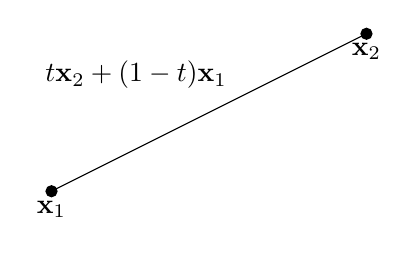
\begin{tikzpicture}
            \draw[fill=black] (0, 0) circle (2pt) node[below] {$\mathbf x_1$};
            \draw[fill=black] (4, 2) circle (2pt) node[below] {$\mathbf x_2$};
            \draw (0, 0) -- (4, 2) node[midway, above left, yshift=5pt, xshift=10pt] {$t \mathbf x_2 + (1 - t) \mathbf x_1$};
          \end{tikzpicture}
        \end{figure}
        \centering\fbox{FTC: $\int_a^b g'(t) dt = g(b) - g(a)$}
      }
      &= \left\lVert \int_0^1 \varphi_{\mathbf y}'(t \mathbf x_2 + (1 - t) \mathbf x_1) \cdot (\mathbf x_2 - \mathbf x_1) dt \right\rVert && \text{chain rule} \\
      &\leq \int_0^1 \underbrace{\lVert \varphi_{\mathbf y}'(t \mathbf x_2 + (1 - t) \mathbf x_1) \cdot (\mathbf x_2 - \mathbf x_1) \rVert}_{\leq \underbrace{\lVert \varphi_{\mathbf y}(\quad) \rVert}_{< \frac{1}{2}} \cdot \lVert \mathbf x_2 - \mathbf x_1 \rVert} dt
      \intertext{
        \begin{figure}[H]
          \centering
          \begin{subfigure}{0.45\textwidth}
            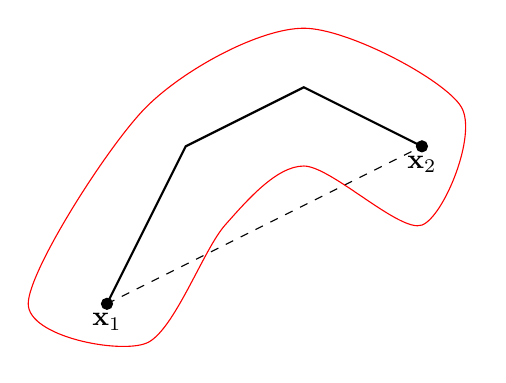
\begin{tikzpicture}
              \draw[fill=black] (0, 0) circle (2pt) node[below] {$\mathbf x_1$};
              \draw[fill=black] (4, 2) circle (2pt) node[below] {$\mathbf x_2$};
              \draw[thick] (0, 0) -- (1, 2) -- (2.5, 2.75) -- (4, 2);
              \draw[dashed] (0, 0) -- (4, 2);
              \draw[red] plot [mark=none, smooth cycle] coordinates {(0.5, -0.5) (1.5, 1) (2.5, 1.75) (4, 1) (4.5, 2.5) (2.5, 3.5) (0.5, 2.5) (-1, 0)};
            \end{tikzpicture}
          \end{subfigure}
          \begin{subfigure}{0.45\textwidth}
            \centering
            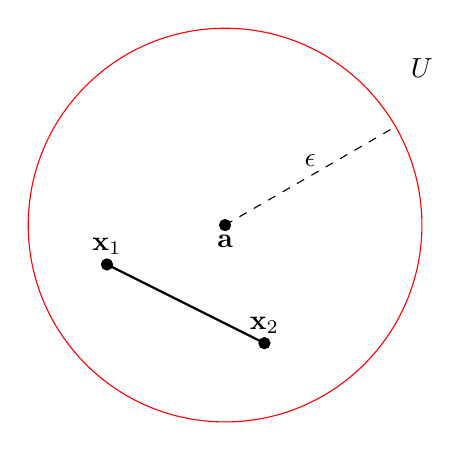
\begin{tikzpicture}
              \draw[red] (0, 0) circle (2.5);
              \node at (2.5, 2) {$U$};
              \draw[fill=black] (0, 0) circle (2pt) node[below] {$\mathbf a$};
              \draw[dashed] (0, 0) -- (30:2.5) node[midway, above] {$\epsilon$};
              \draw[fill=black] (-1.5, -0.5) circle (2pt) node[above] {$\mathbf x_1$};
              \draw[fill=black] (0.5, -1.5) circle (2pt) node[above] {$\mathbf x_2$};
              \draw[thick] (-1.5, -0.5) -- (0.5, -1.5);
            \end{tikzpicture}
          \end{subfigure}
        \end{figure}
      }
      &\leq \frac{1}{2} \lVert \mathbf x_2 - \mathbf x_1 \rVert.
    \end{align*}

    \noindent {\bf Summary:} $\varphi_{\mathbf y} : U \to \RR^n$ is a contraction with $c = \frac{1}{2}$. By CMP, there exists \fbox{at most} one point $\mathbf x \in U$ such that
    \begin{equation} \label{eq:1}
      \varphi_{\mathbf y}(\mathbf x) = \mathbf x \Leftrightarrow \mathbf y = \mathbf f(\mathbf x).
    \end{equation}
    Set $V = \mathbf f(U)$. Then $f : U \to V$ is onto by definition. Further, given any $\mathbf y \in V$, there exists $\mathbf x \in U$ such that
    \[ \mathbf y = \mathbf f(\mathbf x) \Leftrightarrow \text{$\varphi_{\mathbf y}$ has a fixed point $\mathbf x$}. \]
    However, \eqref{eq:1} $\Rightarrow$ $\mathbf x$ is unique; i.e., $\mathbf f : U \xrightarrow{\text{$1$-$1$}} V$ is a bijection.

    \noindent {\bf Exercise:} Check that $V$ is open.
  \end{enumerate}

  (Proof unfinished.)
\end{proof}

\end{document}
